\documentclass{standalone}
\usepackage{pgfplots}
\pgfplotsset{compat=1.15}
\usepackage{mathrsfs}
\usetikzlibrary{arrows, calc}
\newcommand{\degre}{\ensuremath{^\circ}}
\pagestyle{empty}
\begin{document}
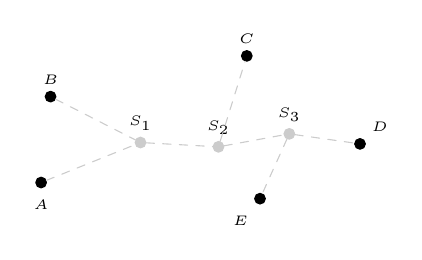
\begin{tikzpicture}[line cap=round,line join=round,x=9cm,y=5.5cm]
    % \clip(-14.126319637473113,-1.645824506401632) rectangle (8.215354312114675,6.424695292648647);

    \begin{tiny}
        \draw(-0.5902366791082465,0.10759522714775753) node[circle,draw, fill=black, scale=0.6] (A) [label={[yshift=-0.5cm]$A$}] {};
        \draw (-0.5769230701353238,0.30596799149252146) node[circle,draw, fill=black, scale=0.6] (B) [label={$B$}] {};

        \draw (-0.3,0.4) node[circle,draw, fill=black, scale=0.6] (C) [label={$C$}] {};
        \draw (-0.14023669368546937,0.19679641713412993) node[circle,draw, fill=black, scale=0.6] (D) [label={[xshift=0.25cm]$D$}] {};
        \draw (-0.2813609509364418,0.07031712226437783) node[circle,draw, fill=black, scale=0.6] (E) [label={[xshift=-0.25cm, yshift=-0.5cm]$E$}] {};

        % Steiner points
        \draw (-0.45,0.2) node[circle,draw=gray!40, fill=gray!40, scale=0.6] (S1) [label={$S_1$}] {};
        \draw (-0.34,0.19) node[circle,draw=gray!40, fill=gray!40, scale=0.6] (S2) [label={$S_2$}] {};
        \draw (-0.24,0.22) node[circle,draw=gray!40, fill=gray!40, scale=0.6] (S3) [label={$S_3$}] {};

        % Edges
        \foreach \source/\target in {A/S1, B/S1, S1/S2, S2/S3, S2/C, S3/D, S3/E} {
                \draw[dashed,gray!40] (\source) -- (\target);
            }
    \end{tiny}
\end{tikzpicture}
\end{document}